% !TEX TS-program = pdflatex

\documentclass[unicode,11pt,notheorems,xcolor=table]{beamer}

\usepackage[T2A]{fontenc}
\usepackage[utf8]{inputenc}
\usepackage[russian]{babel}
\usepackage{amsmath,amsfonts,amssymb,amsthm}
\usepackage{mathtools}
\usepackage{diagbox}

\usepackage{ulem}
\usepackage{tikz}
\usepackage{graphicx}
%\usepackage{tkz-graph}
\usetikzlibrary{matrix,arrows,decorations.pathmorphing, arrows.meta,positioning}
\usetikzlibrary{positioning,calc}
\usetikzlibrary{patterns}
\usetikzlibrary{decorations.pathreplacing}

%Описание стиля презентации
\usetheme[sidebar=0]{kfmn} 
\setbeamercovered{transparent}

%\definecolor{cyan}{RGB}{240,217,1}
%\definecolor{vgugreen}{RGB}{143,188,103}
%\definecolor{vgured}{RGB}{234,38,40}
%\definecolor{vgublue}{RGB}{53,101,167}
\hypersetup{colorlinks,linkcolor=,urlcolor=blue}

\makeatletter
	\g@addto@macro{\endtabular}{\rowfont{}}% Clear row font
	\makeatother
	\newcommand{\rowfonttype}{}% Current row font
	\newcommand{\rowfont}[1]{% Set current row font
		\gdef\rowfonttype{#1}#1\ignorespaces%
	}
\makeatother

\newcommand{\myunit}{9mm}
\tikzset{
    node style sp/.style={draw,circle,minimum size=\myunit},
    node style ge/.style={circle,minimum size=\myunit},
    arrow style mul/.style={draw,sloped,midway,fill=white},
    arrow style plus/.style={midway,sloped,fill=white},
}

%[0, 6, 8, 8, 10, 5, 6, 10, 8, 10, 10], 

\pgfdeclareimage[height=8mm]{university-logo}{logo-iem.png}
\logo{\pgfuseimage{university-logo}}
%2[0, 11, 10, 8, 11, 5, 11, 11, 8, 11, 10, 11],

\titlepicture{
	\begin{tikzpicture}[y=1.4cm,overlay,rotate=8]
	\coordinate (O) at (-3cm,0.9cm);
	\filldraw[thick,draw= vgublue, fill=vgublue!20!white] (0,0) circle[radius=4.2cm];
	\clip (0,0) circle[radius=4.2cm];
	\draw (-1.5,1.5) node{
	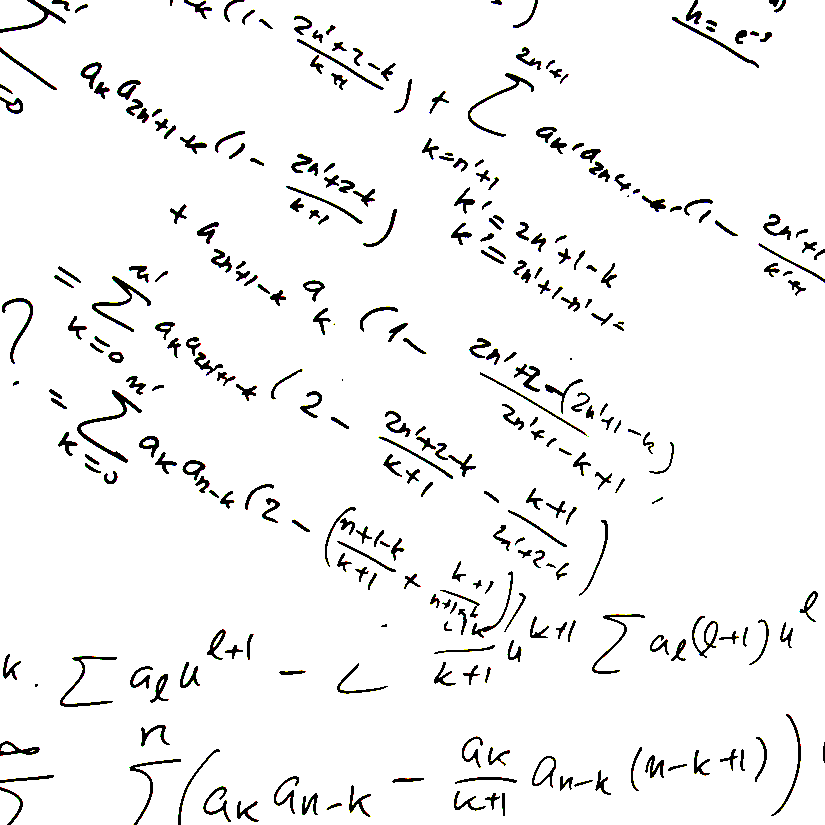
\includegraphics[width=8cm]{titlepic.png}
	};
\end{tikzpicture}
}

\usepackage[math]{iwona}

\newcommand{\hplus}{\mathbin{\hat+}}
\newcommand{\hdot}{\mathbin{\hat\cdot}}
% Описание теорем
\newtheorem{theorem}{Теорема}
\newtheorem{seq}{Следствие}
%%

\LECT % 

% Титульный лист теорем
\author[Д.\,В. Чупраков]{канд.\,физ.-матем.\,наук, доцент Д.\,В. Чупраков\\[6pt] usr10381@vyatsu.ru}

\institute[ВятГУ]{ФГБОУ ВО Вятский государственный университет}

\department{Факультет экономики и финансов}

\title[Лекция~14. Дискретные случайные величины]{
	Введение в экономико-математическое моделирование\\[12pt]
	Лекция~14. Дискретные случайные величины}
\date{9 декабря 2020~г.}


\setbeamercovered{invisible}

\setbeamercolor{math text}{fg=vgured!70!black}


\begin{document}


\maketitle

\begin{frame}{Структура лекции}{}
	\tableofcontents
\end{frame}

\section{Случайные величины}
\subsection{Определение}


\begin{frame}{Дискретная случайная величина}{}
    Пусть 
    \begin{itemize}
        \item $\Omega$~--- пространство элементарных событий некоторого опыта, 
        \item $X$~--- конечное или счетное  числовое множество.
    \end{itemize}

    \begin{block}{Определение}
    Функция, сопоставляющая каждому исходу пространства $\Omega$ некоторый элемент множества $X$, называется \alert{дискретной случайной величиной.}
    $$
        X = X(\omega),\quad \omega \in \Omega
    $$
    \end{block}

    \alert{Событие} связанное со случайной величиной $X$~--- любое подмножество ее множества значений.
\end{frame}

\begin{frame}{Примеры случайных величин}{}
    
    \begin{itemize}
        \item Опыт с подбрасыванием игральной кости. 
        \begin{itemize}
            \item Событие $\omega$~--- положение игральной кости 
            \item Величина $X$~--- ,,число очков, выпавших при однократном подбрасывании кости``.
        \end{itemize}
        
        \item Опыт с магазином. 
        \begin{itemize}
            \item Событие $\omega$~--- посещение магазина очередным покупателем.
            \item Величина $Y = Y(\omega)$~--- ,,число покупателей в магазине в течение часа``.
        \end{itemize}
    \end{itemize}
\end{frame}


\subsection{Закон распределения}

\begin{frame}{Закон распределения}{}
    Предположим, $X = X(\omega)$~--- дискретная случайная величина, значениями которой являются числа
    $$
        x_1 = X(\omega_1), x_2= X(\omega_2),\ldots, x_n = X(\omega_n),\ ldots
    $$
    
    Сопоставим каждому $x_i$ вероятность 
    $$
    p_i = p(X=x_i) = p(\omega_i).
    $$ 

    Сумма вероятностей всех значений случайной величины равна единице:
    $$
        p_1 + p_ 2 + \ldots + p_n = 1.
    $$
    
    \begin{block}{Определение}
        Отображение, при котором каждому возможному значению дискретной случайной величины соответствует вероятность события, при котором случайная величина принимает это значение, называется \alert{законом распределения дискретной случайной величины.}
    \end{block}
    
    Закон распределения можно задать в виде
    \begin{itemize}
        \item таблицы, 
        \item графика, 
        \item формулы.
    \end{itemize}
\end{frame}


\begin{frame}{Табличная форма закона распределения}{}
    \begin{block}{}
    Каждая таблица 

    $$
        \begin{array}{c|cccc}
            x_i & x_1 & x_2 & \ldots & x_n \\
            \hline
            p_i & p_1 & p_2 & \ldots & p_n \\
        \end{array},
        \qquad
        p_1+p_2+\ldots+p_n=1
    $$
    задает некоторую дискретную случайную величину.
    
    При этом $p(X=x_i)=p_i$
    \end{block}

    

    \begin{tikzpicture}[y=2.3mm,>=latex]
        \small
        \draw (-0.5,0) -- (4,0);
        \draw[dashed] (4,0) -- (6,0);
        \draw[->] (6,0) -- (8,0) node[right]{$x_i$};
        \draw[->] (0,-0.5) -- (0, 7) node[left]{$p_i$};
        \draw
             (0,0)  node[below left]{0}
        ;
        \path
            (1, 2.5) coordinate (A1)
            (2, 0.5) coordinate (A2)
            (4, 3.4) coordinate (A3)
            (6, 1.3) coordinate (A4)
        ;

        \draw
            ($(0,0)!(A1)!(5,0)$) +(0,0.2) -- +(0,-0.2) node[below]{$x_1$}
            ($(0,0)!(A2)!(5,0)$) +(0,0.2) -- +(0,-0.2) node[below]{$x_2$}
            ($(0,0)!(A3)!(5,0)$) +(0,0.2) -- +(0,-0.2) node[below]{$x_3$}
            ($(0,0)!(A4)!(5,0)$) +(0,0.2) -- +(0,-0.2) node[below]{$x_n$}
        ;
        \draw
            ($(0,0)!(A1)!(0,5)$) +(0.1,0) -- +(-0.1,0) node[left]{$p_1$}
            ($(0,0)!(A2)!(0,5)$) +(0.1,0) -- +(-0.1,0) node[left]{$p_2$}
            ($(0,0)!(A3)!(0,5)$) +(-0.1,0) -- +(0.1,0) node[right]{$p_3$}
            ($(0,0)!(A4)!(0,5)$) +(-0.1,0) -- +(+0.1,0) node[right]{$p_n$}
            (0,6) +(0.1,0) -- +(-0.1,0) node[left]{$1$}
        ;
          \draw[thick,draw=vgublue] 
          (A1)-- (A2) -- (A3) ;
          \draw[thick,draw=vgublue,dashed] 
            (A3) -- (A4);
         \fill[fill=vgublue] 
            (A1) circle[radius = 2pt]
            (A2) circle[radius = 2pt]
            (A3) circle[radius = 2pt]
            (A4) circle[radius = 2pt];
    \end{tikzpicture}
    \begin{block}{}
        График закона распределения называется \alert{многоугольником распределения}
    \end{block}
\end{frame}

\begin{frame}[allowframebreaks]{Пример}{}
    \begin{exampleblock}{Пример}
        Делопроизводитель написал три письма и подписал три конверта. 
        Его помощник, не задумываясь о содержании писем, разложил их по конвертам  писем и отправил.
        Составьте закон распределения величины $X$~--- число человек, получивших адресованные именно им письма.
    \end{exampleblock}
    \begin{itemize}
        \item Определим значения случайной величины $X$:
        \begin{itemize}
            \item $X = 0$, если ни один из адресатов не получил своё письмо.
            \item $X = 1$, если только один из адресатов получил своё письмо.
            \item $X = 2$, если только два адресата получили свои письма.
            \item $X = 3$, если все адресаты получили свои письма.
        \end{itemize}
        \item Письма можно разложить по конвертам
        $P_3 = 3\cdot 2 \cdot 1 = 6~\text{способами}$
        \item  $X=3$ можно получить одним способом: $P(X=3)=\frac{1}{6}$
        $$
        \begin{array}{c|c|c}
            1 & 2& 3\\
            \hline
            1 & 2& 3\\
        \end{array}
        $$
        \item  $X=2$ не наступит никогда: $P(X=2)=0$;
        \item  $X=1$ наступает в трех случаях $P(X=1)=\frac{3}{6}-\frac{1}{2}$:
        $$
        \begin{array}{c|c|c}
            1 & 2& 3\\
            \hline
            1 & 3& 2\\
        \end{array}
        \quad
        \begin{array}{c|c|c}
            1 & 2& 3\\
            \hline
            3 & 2& 1\\
        \end{array}
        \quad
        \begin{array}{c|c|c}
            1 & 2& 3\\
            \hline
            2 & 1& 3\\
        \end{array}
        $$
        \item  $X=0$ наступает в трех случаях: $P(X=0)=\frac{2}{6}=\frac{1}{3}$
        $$
        \begin{array}{c|c|c}
            1 & 2& 3\\
            \hline
            3 & 1& 2\\
        \end{array}
        \quad
        \begin{array}{c|c|c}
            1 & 2& 3\\
            \hline
            2 & 3& 1\\
        \end{array}
        $$
        \item Составим закон распределения:
        $$
        \begin{array}{c|cccc}
            x_i& 0 &1 & 2& 3\\
            \hline
            p_i & \dfrac{1}{3} & \dfrac{1}{2}& 0 & \dfrac{1}{6}\\
        \end{array}
        $$
        \item Проверим корректность
        $$
            \sum_{i=1}^4 p_i = \frac{1}{3}+\frac{1}{2}+0+\frac{1}{6}=1
        $$
        \item Построим многоугольник распределения:
        \begin{tikzpicture}[y=6mm,>=latex]
            \draw[->] (-0.5,0) -- (8,0) node[right]{$x_i$};
            \draw[->] (0,-0.5) -- (0, 7) node[left]{$p_i$};
            \draw
                 (0,0)  node[below left]{0}
            ;
            \draw
                 (2,0) +(0,0.2) -- +(0,-0.2) node[below]{1}
                 (4,0) +(0,0.2) -- +(0,-0.2) node[below]{2}
                 (6,0) +(0,0.2) -- +(0,-0.2) node[below]{3}
            ;
            \draw
                 (0,1) +(0.1,0) -- +(-0.1,0) node[left]{1/6}
                 (0,2) +(0.1,0) -- +(-0.1,0) node[left]{1/3}
                 (0,3) +(0.1,0) -- +(-0.1,0) node[left]{1/2}
                 (0,4) +(0.1,0) -- +(-0.1,0) node[left]{2/3}
                 (0,5) +(0.1,0) -- +(-0.1,0) node[left]{5/6}
                 (0,6) +(0.1,0) -- +(-0.1,0) node[left]{1}
            ;
            \path
                (0, 2) coordinate (A1)
                (2, 3) coordinate (A2)
                (4, 0) coordinate (A3)
                (6, 1) coordinate (A4)
            ;
             \draw[dashed,draw=black!40] 
                ($(0,0)!(A2)!(5,0)$) -- (A2) -- ($(0,0)!(A2)!(0,5)$)
                ($(0,0)!(A4)!(5,0)$) -- (A4) -- ($(0,0)!(A4)!(0,5)$);
             \draw[thick,draw=vgured] 
             (A1)-- (A2) -- (A3) -- (A4);
             \fill[fill=vgured] 
                (A1) circle[radius = 2pt]
                (A2) circle[radius = 2pt]
                (A3) circle[radius = 2pt]
                (A4) circle[radius = 2pt];
        \end{tikzpicture}
    
    \end{itemize}
    
\end{frame}

\begin{frame}{Функция распределения}{}

    \begin{block}{Определение} 
        \alert{Функцией распределения} случайной величины называется функция
        $$
        F(x) = p(X < x).
        $$
        \begin{itemize}
            \item определенная на $(-\infty; + \infty)$;
            \item принимающая каждой точке $x$ значение вероятности события ,, Значение случайной величины меньшее, чем $x$``. 
        \end{itemize}
        
        
    \end{block}
        \structure{Геометирческий смысл}

        % Функция распределения определяет вероятность того, что случайная величина $X$ в результате исхода попадет на координатную прямую левее $x$:
        {\centering
        \begin{tikzpicture}[x=15mm]
            \draw[->]  
                (0,0) -- (5,0) node[below]{$X$}
            ;
            \path[pattern=north west lines] (0,0) rectangle (4,0.2) ;
            \path[pattern=north east lines] (0,0) rectangle (2,-0.2) 
            ;
            \draw
                (4,0)  + (0,+0.1) -- +(0,-0.1) node[below] {$x_2$}
                (2,0)  + (0,+0.1) -- +(0,-0.1) node[below] {$x_1$}
                (1,-0.5) node{$F(x_1)$}
                (2.5,0.5) node{$F(x_2)$}
            ;
        \end{tikzpicture}
        \par}

\end{frame}

\begin{frame}{Функция распределения ДСВ}{}
\begin{block}{}
 Для ДСВ $X$, значения которой $x_1, x_2,\ldots, x_n$
  функция распределения имеет вид 
  
  $$
    f(x) = \sum_{x_k<x} p(X=x_k)
  $$
\end{block}

Вычислим значения функции распределения $F(x)$

 \begin{itemize}
     \item  При $x \leqslant x_1 $\hfill$F (x) = P (X < x) = 0$.
     \item  При $ x_1< x \leqslant x_2 $\hfill $F (x) = P (X < x) = P(X=x_1)=p_1$.
     \item  При $ x_2< x \leqslant x_3 $\hfill 
     $F (x) = P (X < x) = p_1+p_2$.
     \item  При $ x_{n-1}< x \leqslant x_n $\hfill $F (x) = p_1+p_2+ \ldots + p_{n-1}$.
     \item При $ x >x_n$ \hfill $F (x) = P (X < x) = 1$.
 \end{itemize}
\end{frame}

\begin{frame}[allowframebreaks]{Функция распределения ДСВ и ее график}{}
\begin{exampleblock}{Пример}
    Рассмотрим закон распределения
    \quad $
    \begin{array}{c|cccc}
        x_i& 0 &1 & 2& 3\\
        \hline
        p_i & \dfrac{1}{3} & \dfrac{1}{2}& 0 & \dfrac{1}{6}\\
    \end{array}
    $\\
    и построим функцию распределения $F(x)$:
\end{exampleblock}


    \begin{itemize}
        \item $x\leqslant 0$: 
        $$F(x)= p(X<x) = 0$$
        
        % \vspace{-3ex}
        \item $0<x\leqslant 1$: $$F(x)= p(X<x) = p(X=0) = \frac{1}{3}$$
        
        % \vspace{-3ex}
        \item $1<x\leqslant 2$: $$F(x)= p(X<x) = p(X\in \{0,1\}) = \frac{1}{3}+\frac{1}{2}= \frac{5}{6}$$
        
        % \vspace{-3ex}
        \item $2<x\leqslant 3$: $$F(x)= p(X<x) = p(X\in \{0,1,2\}) = \frac{1}{3}+\frac{1}{2} + 0= \frac{5}{6}$$
        
        % \vspace{-3ex}
        \item  $x>3$: $$F(x)= p(X<x) = p(X\in \{0,1,2,3\}) = 1$$

    \end{itemize}
    
    \framebreak

    Функция распределения имеет вид:
    $$
    F(x) = \begin{cases}
        0, &  x \leqslant 0,\\
        1/3, &  0<x \leqslant 1,\\
        5/6, &  0<x \leqslant 3,\\
        1, &  3<x. \\
        \end{cases}
    $$

    Ее график:
    \begin{tikzpicture}[x=10mm,y=3.6mm,>=latex]
        \draw[->] (-2,0) -- (8,0) node[right]{$x$};
        \draw[->] (0,-1) -- (0, 7) node[right]{$F(x)$};
        \draw
             (0,0)  node[below left]{0}
        ;
        \draw
             (2,0) +(0,0.2) -- +(0,-0.2) node[below]{1}
             (4,0) +(0,0.2) -- +(0,-0.2) node[below]{2}
             (6,0) +(0,0.2) -- +(0,-0.2) node[below]{3}
        ;
        \draw
             (0,1) +(0.1,0) -- +(-0.1,0) node[left]{}
             (0,2) +(0.1,0) -- +(-0.1,0) node[left]{1/3}
             (0,3) +(0.1,0) -- +(-0.1,0) node[left]{}
             (0,4) +(0.1,0) -- +(-0.1,0) node[left]{}
             (0,5) +(0.1,0) -- +(-0.1,0) node[left]{5/6}
             (0,6) +(0.1,0) -- +(-0.1,0) node[left]{1}
        ;
        \draw[very thick,draw=vgublue] 
            (-3,0) -- (0,0)
            (0,2) -- (2,2)
            (2,5) -- (6,5)
            (6,6) -- (8,6);
        \fill[fill=vgublue] 
            (0,0) circle[radius=3pt]
            (2,2) circle[radius=3pt]
            (6,5) circle[radius=3pt]
        ;
        \fill[draw=vgublue, fill=white,very thick] 
            (0,2) circle[radius=3pt]
            (2,5) circle[radius=3pt]
            (6,6) circle[radius=3pt]
        ;
    \end{tikzpicture}

\end{frame}

\begin{frame}{Свойства функции распределения}{}

    \begin{itemize}
        \item $0 \leqslant F(x) \leqslant 1$
        \item $F(x)$ не убывающая: $ x_1<x_2 \Rightarrow F(x_1) \leqslant F(x_2)$;
        \item $\lim\limits_{x\to -\infty} F(x) = 0$;
        \item $\lim\limits_{x\to +\infty} F(x) = 1$;
    \end{itemize}

    \begin{block}{}
        Вероятность попадания случайной величины $X$ в интервал $(a,b)$ равна разности значений функции распределения в правом и левом концах интервала:
        $$
            P(a < X < b)=F(b)-F(a)
        $$
    \end{block}
\end{frame}

% \begin{frame}{}{}
 
% \end{frame}

% \begin{frame}{}{}

% \end{frame}

% \begin{frame}{}{}

% \end{frame}

% \begin{frame}{}{}

% \end{frame}

% \begin{frame}{}{}

% \end{frame}

% \begin{frame}{}{}

% \end{frame}

\section{Операции над случайными величинами}
\subsection{Сложение случайных величин}

\begin{frame}{Независимые случайные величины}{}

    \begin{block}{Определение}
        Две случайные величины называются \alert{независимыми}, если закон распределения одной из них не меняется от того, какие возможные значения приняла другая величина.
    \end{block}

    % Так, если дискретная случайная величина X может принимать значения лг; (г = 1, 2, ..., п), а случайная величина У — значения У} (/=1,2, ..., т), то независимость дискретных случайных величин X и У означает независимость событий X = х{ и У = уу при любых ? = 1,2, ..., п и у=1,2, ..., т. В противном случае случайные величины называются зависимыми.

    % Например, если имеются билеты двух различных денежных лотерей, то случайные величины X и У, выражающие соответственно выигрыш по каждому билету (в денежных единицах), будут независимыми, так как при любом выигрыше по билету одной лотереи (например, при Х = х{) закон распределения выигрыша по другому билету (У) не изменится. Если же случайные величины X и У выражают выигрыш по билетам одной денежной лотереи, то в этом случае X и У являются зависимыми, ибо любой выигрыш по одному билету (X=х{) приводит к изменению вероятностей выигрыша но другому билету (У), т.е. к изменению закона распределения У.
    
   
\end{frame}
\begin{frame}{Умножение ДСВ на число}{}
    
    %  Пусть даны две случайные величины $X$, $Y$:
    
     \begin{block}{Определение}
        \alert{Произведением $kX$ случайной величины $X$ на постоянную величину $k$} называется случайная величина, которая принимает значения $kx_i$ с теми же вероятностями $p_i$.
     \end{block}

     \bigskip
     \structure{Пример:}

     \medskip

     Пусть 
     $$
     X\colon \begin{array}{|c|ccc|}
        \hline
         x_i & -2 & 1& 2 \\
         \hline
         p_i & 0.5 & 0.3 & 0.2 \\
         \hline
        \end{array}
     $$
    
    Тогда $Y=3X$ имеет вид
    $$
   Y\colon \begin{array}{|c|ccc|}
       \hline
        y_i & -6 & 3& 6 \\
        \hline
        p_i & 0.5 & 0.3 & 0.2 \\
        \hline
       \end{array}
    $$
   
\end{frame}

\begin{frame}{Степень  ДСВ}{}
    
    %  Пусть даны две случайные величины $X$, $Y$:
    
     \begin{block}{Определение}
        \alert{$n$-й степенью} случайной величины $X$, называется случайная величина $X^n$, которая принимает значения $x_i^n$ с теми же вероятностями $p_i$
     \end{block}

    \bigskip
    \structure{Пример:}

    \medskip
    \begin{itemize}
        \item Пусть \hfill
        $
        X\colon \begin{array}{|c|ccc|}
           \hline
            x_i & -2 & 1& 2 \\
            \hline
            p_i & 0.5 & 0.3 & 0.2 \\
            \hline
           \end{array}
        $
        \item Тогда $Y=X^2$ имеет вид\hfill
        $
       Y\colon \begin{array}{|c|ccc|}
           \hline
            y_i & 4 & 1& 4 \\
            \hline
            p_i & 0.5 & 0.3 & 0.2 \\
            \hline
           \end{array}
        $
        \item По теореме о сумме несовместных событий: 
        \\~\hfill$
       Y\colon \begin{array}{|c|cc|}
           \hline
            y_i &  1& 4 \\
            \hline
            p_i & 0.3 & 0.7 \\
            \hline
           \end{array}
        $

     \end{itemize}
\end{frame}


\begin{frame}{Сумма и произведение независимых ДСВ}{}
    \begin{block}{Определение}
        \alert{Суммой} независимых ДСВ~$X$ и~$Y$ называется случайная величина $Z=X+Y$, которая принимает все возможные значения вида $z_{ij} = x_i+y_j$ с вероятностями 
        $$
            p_{ij}=P( (X=x_i)\cdot(Y=y_j)) = p_i\cdot p'_j
        $$
     \end{block}


     \begin{block}{Определение}
        \alert{Произведением} независимых ДСВ~$X$ и~$Y$ называется случайная величина $Z=X \cdot Y$, которая принимает все возможные значения вида $z_{ij} = x_i \cdot y_j$ с вероятностями 
        $$
            p_{ij}=P( (X=x_i)\cdot(Y=y_j)) = p_i\cdot p'_j
        $$
     \end{block}
\end{frame}

\begin{frame}{Пример вычисления суммы ДСВ}{}
    \begin{exampleblock}{}
        Даны ДСВ
        $X\colon \begin{array}{|c|ccc|}
        \hline
         x_i & -2 & 1& 2 \\
         \hline
         p_i & 0.5 & 0.3 & 0.2 \\
         \hline
        \end{array}
        \qquad
        Y\colon \begin{array}{|c|ccc|}
            \hline
             y_i & 0 & 2& 4 \\
             \hline
             p'_i & 0.1 & 0.6 & 0.3 \\
             \hline
            \end{array}
        $
        
        \smallskip
        Вычислить сумму $Z=X+Y$.
    \end{exampleblock}
    
    \vspace{-6mm}
    \begin{gather*}
        \begin{array}{|c|ccc|}
            \multicolumn{4}{c}{x_i+y_j}\\
            \hline
            \text{\diagbox{$x_i$}{$y_j$}} & 0 & 2 & 4 \\
            \hline
            -2 & -2 & 0 & \cellcolor{yellow!40} 2 \\
            1 &  1 & 3 & 5 \\
            2 & \cellcolor{yellow!40} 2 & 4 & 6 \\
            \hline
        \end{array}
        \qquad
        \begin{array}{|c|ccc|}
            \multicolumn{4}{c}{p_{ij}=p_i\cdot p'_j}\\
            \hline
            \text{\diagbox{$p_i$}{$p'_j$}} & 0.1 & 0.6 & 0.3 \\
            \hline
            0.5 & 0.05 & 0.3 & \cellcolor{yellow!40} 0.15 \\
            0.3 &  0.03 & 0.18 & 0.09 \\
            0.2 & \cellcolor{yellow!40} 0.02 & 0.12 & 0.06 \\
            \hline
        \end{array}
        \\[5pt]
        p(Z=2) = 0.15+0.02=0.17
        \\[5pt]
        X+ Y \colon\begin{array}{|c|cccccccc||c|}
            \hline
            z_i & -2 & 0 & 1 & 2 & 3 & 4 & 5& 6 & \Sigma\\
            p_i & 0.05 & 0.3 & 0.03 & 0.17 & 0.18 &  0.12 & 0.09 & 0.06 & 1\\
            \hline
        \end{array}
    \end{gather*}
\end{frame}

\begin{frame}{Пример вычисления произведения ДСВ}{}
    \begin{exampleblock}{}
        Даны ДСВ
        $X\colon \begin{array}{|c|ccc|}
        \hline
         x_i & -2 & 1& 2 \\
         \hline
         p_i & 0.5 & 0.3 & 0.2 \\
         \hline
        \end{array}
        \qquad
        Y\colon \begin{array}{|c|ccc|}
            \hline
             y_i & 0 & 2& 4 \\
             \hline
             p'_i & 0.1 & 0.6 & 0.3 \\
             \hline
            \end{array}
        $

        \smallskip
        Вычислить произведение $Z=X\cdot Y$.
    \end{exampleblock}
    
    \vspace{-6mm}
    \begin{gather*}
        \begin{array}{|c|ccc|}
            \multicolumn{4}{c}{x_i \cdot y_j}\\
            \hline
            \text{\diagbox{$x_i$}{$y_j$}} & 0 & 2 & 4 \\
            \hline
            -2 & \cellcolor{yellow!40} 0 & -4 & -8 \\
             1 & \cellcolor{yellow!40} 0 & 2 & \cellcolor{cyan!20} 4 \\
             2 & \cellcolor{yellow!40} 0 & \cellcolor{cyan!20} 4 & 8 \\
            \hline
        \end{array}
        \qquad
        \begin{array}{|c|ccc|}
            \multicolumn{4}{c}{p_{ij}=p_i\cdot p'_j}\\
            \hline
            \text{\diagbox{$p_i$}{$p'_j$}} & 0.1 & 0.6 & 0.3 \\
            \hline
            0.5 & \cellcolor{yellow!40} 0.05 & 0.3 & 0.15 \\
            0.3 & \cellcolor{yellow!40}  0.03 & 0.18 & \cellcolor{cyan!20} 0.09 \\
            0.2 & \cellcolor{yellow!40}  0.02 & \cellcolor{cyan!20} 0.12 & 0.06 \\
            \hline
        \end{array}
        \\[5pt]
        p(Z=0) = 0.05+0.03+0.02=0.1
        \\
        p(Z=4) = 0.09+0.12=0.21
        \\[5pt]
        XY \colon\begin{array}{|c|cccccc||c|}
            \hline
            z_i & -8 & -4 & 0 & 2 & 4 & 8  & \Sigma\\
            p_i & 0.15 & 0.3 & 0.1 & 0.18 & 0.21 &  0.06 & 1\\
            \hline
        \end{array}
    \end{gather*}
\end{frame}
 

\section{Числовые характеристики случайных величин}

\begin{frame}{}{}
    {\centering \bfseries \Large Числовые характеристики \\случайных величин\par}
\end{frame}
\begin{frame}[t]{Мода и медиана}{}
    \begin{block}{Определение}
        \alert{Мода $Mo(X)$}~--- значение случайной величины $X$, имеющей максимальную вероятность.
    \end{block}
    
    В зависимости от вида распределения случайная величина может иметь разное количество мод. 
    
    \begin{itemize}
        \item Распределение \alert{одномодальное}, если мода одна
        \item Распределение \alert{двумодальное}, если моды две
        \item Распределение \alert{мультимодальное}, если   мод больше двух.
    \end{itemize}


\end{frame}

\begin{frame}{Математическое ожидание}{}
    \begin{block}{Определение}
    \alert{Математическим ожиданием} $M(X)$ называют сумму произведений всех возможных значений случайной величины $x_i$ на соответствующие вероятности $p_i$:               
    $$
        M(X) = x_1\cdot p_1 + x_2 \cdot p_2 + \ldots + x_n \cdot p_n = \sum_{i=1}^n x_i p_i
    $$
    \end{block}

    Математическое ожидание~--- это среднее значение случайной величины $X$, которое следует ожидать в результате многократного проведения опыта.
\end{frame}

\begin{frame}{Пример}
    \begin{exampleblock}{}
        Закон распределения случайной величины $X$ задан таблицей:
        $$
        \begin{array}{|c|cccc|}
            \hline
            x_i & -5 & 0 & 2 & 6 \\
            p_i & 0.1 & 0.2 & 0.3 & 0.4\\
            \hline
        \end{array}
        $$
        Вычислить математическое ожидание $X$.
    \end{exampleblock}

    \begin{itemize}
        \item Добавим в таблицу строку $x_ip_i$ и столбец $\Sigma$
        $$
        \begin{array}{|c|cccc||c|}
            \hline
            x_i & -5 & 0 & 2 & 6 & \Sigma\\
            p_i & 0.1 & 0.2 & 0.3 & 0.4 & 1\\
            \hline
            \hline
            x_ip_i & -0.5 & 0 & 0.6 & 2.4 & \cellcolor{yellow!40} 2.5\\
            \hline
        \end{array}
        $$

        \item Каждое значение третьей строки~--- произведение $x_i\cdot p_i$.
        \item $M(X)= x_1p_1+x_2p_2+x_3p_3+x_4p_4 = -0.5+0+0.6+2.4=2.5$
    \end{itemize}
\end{frame}


\begin{frame}{Свойства математического ожидания}{}
    \begin{block}{}
    $$
        M(X) = x_1\cdot p_1 + x_2 \cdot p_2 + \ldots + x_n \cdot p_n = \sum_{i=1}^n x_i p_i
    $$
    \end{block}
    \begin{enumerate}
        \item  $M(C) = C$, \hfillесли $C$~--- константа;
        \item  $M(kX) = k\cdot M(x)$, \hfill если $k$~--- константа;
        \item $M(X \pm Y) = M(X) \pm M(Y)$;
        \item $M(XY) = M(X) \cdot M(Y)$,\hfill если $X$, $Y$~--- независимые СВ.
    \end{enumerate}
\end{frame}


\begin{frame}{Дисперсия}{}
    \begin{block}{}
    Дисперсией случайной величины $X$ называют математическое ожидание квадрата ее отклонений от среднего значения:
    $$
        D(X) = \sum_{i=1}^n (x_i-M(X))^2p_i
    $$
    \end{block}

    \begin{itemize}
        \item Дисперсия характеризует степень отклонения значений случайной величины от ее среднего значения. 
        \item Чем больше дисперсия, тем большую случайность проявляет величина.
        \item На практике дисперсия служит для оценки меры риска.
    \end{itemize}
\end{frame}



\begin{frame}{Пример}
    \begin{exampleblock}{}
        Закон распределения случайной величины $X$ задан таблицей:

        $$
        \begin{array}{|c|cccc|}
            \hline
            x_i & -5 & 0 & 2 & 6 \\
            p_i & 0.1 & 0.2 & 0.3 & 0.4\\
            \hline
        \end{array}
        $$
        Вычислить дисперсию $X$.\par
    \end{exampleblock}

    \begin{itemize}
        \item Добавим в таблицу строки $x_ip_i$, $x^2p_i$ и столбец $\Sigma$

        $$
        \begin{array}{|c|cccc||c|}
            \hline
            x_i & -5 & 0 & 2 & 6 & \Sigma\\
            p_i & 0.1 & 0.2 & 0.3 & 0.4 & 1\\
            \hline
            \hline
            x_ip_i & -0.5 & 0 & 0.6 & 2.4 & \cellcolor{yellow!40} 2.5=M(X)\\
            x^2_ip_i & 2.5 & 0 & 1.2 & 14.4 & \cellcolor{yellow!40} 18.1=M(X^2)\\
            \hline
        \end{array}
        $$
        
        % \item Сумма элементов третьей строки~--- $M(X) = 2.5$
        % \item Сумма элементов четвертой строки~--- $M(X^2) = 18.1$
        \item Дисперсия равна $D(X)=M(X^2)-(M(X))^2 = 18.1-2.5^2=11.85$
    \end{itemize}
\end{frame}

\begin{frame}{Свойства дисперсии}{}
    Вычисление дисперсии удобно выполнять по формуле:
    \begin{block}{}
        $$
            D(X) = M(X^2)-(M(X))^2
        $$
    \end{block}

    \structure{Свойства:}
    \begin{itemize}
        \item $D(C) = 0$, \hfillесли $C$~--- константа;
        \item  $D(kX) = |k|\cdot D(X)$, \hfill если $k$~--- константа;
        \item $D(X \pm Y) = D(X) + D(Y)$,\hfill если $X$, $Y$~--- независимые СВ.
    \end{itemize}
    
\end{frame}

\begin{frame}{Среднее квадратическое отклонение}{}
    Дисперсия имеет размерность квадрата случайной величины.
    
    Для того, чтобы оценка рассеяния значений случайной величины была соизмерима с~самой величиной, вычисляют среднеквадратичное отклонение.

    \begin{block}{Определение}
 
    Средним квадратическим отклонением (стандартным отклонением) называется арифметический квадратный корень из дисперсии случайной величины:
    $$
        \sigma(X) = \sqrt{D(X)}
    $$
    \end{block}
\end{frame}

\begin{frame}[allowframebreaks]{Пример}{}
    \begin{exampleblock}{}
        Прибыльность двух инвестиционных проектов Х, Y (млн. руб) задана законами распределения:
        $$
            X\colon\begin{array}{|c|ccc|}
                \hline
                x_i & -1 & 2 & 5 \\
                p_i & 0.2 & 0.6 & 0.2\\
                \hline
            \end{array}
            \qquad
            Y\colon\begin{array}{|c|ccc|}
                \hline
                y_i & -5 & 6 & 10 \\
                p_i & 0.4 & 0.5 & 0.1\\
                \hline
            \end{array}           
        $$
        Какой инвестиционный проект целесообразно выбрать для реализации?
    \end{exampleblock}
    \begin{itemize}
        \item Вычислим характеристики обоих проектов:
        $$
            X\colon\begin{array}{|c|ccc||c|}
                \hline
                x_i & -1 & 2 & 5  & \Sigma\\
                p_i & 0.2 & 0.6 & 0.2 & 1\\
                \hline
                x_ip_i & -0.2 & 1.2 & 1 & 2\\
                x^2_ip_i & 0.2 & 2.4 & 5 & 7.6\\
                \hline
            \end{array}
        $$
        $$
            Y\colon\begin{array}{|c|ccc||c|}
                \hline
                y_i & -5 & 6 & 10 & \Sigma\\
                p_i & 0.4 & 0.5 & 0.1 & \\
                \hline                
                y_ip_i & -2 & 3 & 1 & 2\\
                y^2_ip_i & 10 & 18 & 10 & 38\\
                \hline
            \end{array}           
        $$    
        \begin{align*}
            M(X) &= 2 & D(X) &= 7.6-2^2=3.6 & \sigma(X) &=  \sqrt{3.6} \approx 1.90\\
            M(Y) &= 2 & D(Y) &= 38-2^2=34 & \sigma(Y) &=  \sqrt{34} \approx 5.84\\
        \end{align*}
        \item Математические ожидания величин одинаковые, значит проекты принесут в среднем равный доход.
        \item Среднее квадратичное отклонение второго проекта выше, чем у первого, тем самым риск выше.
    \end{itemize}
    
\end{frame}

% \end{document}


\section{Законы распределения случайных величин}
% \subsection{Равномерное дискретное распределение.}


\subsection{Биномиальный закон распределения}

\begin{frame}{}{}
    {\centering \bfseries \Large Биномиальный закон \\распределения вероятностей\par}
\end{frame}

\begin{frame}{Повторение испытаний}{}
    \begin{itemize}
        \item 
            Пусть дискретная случайная величина $X$~--- количество ,,успехов`` в последовательности из $n$ независимых случайных экспериментов, таких что вероятность ,,успеха`` в каждом из них постоянна и равна $p$.
        \item Величина $X$ может принять любое значение от $0$ до $n$
        \item $\displaystyle  p(X=x_i) = C_n^{x_i} p^{x_i} (1-p)^{n-x_i}$
    \end{itemize}
    \begin{block}{}
    Если значения ДСВ $X$ являются всевозможными числами появления заданного события  при фиксированном числе независимых испытаний, то $X$ имеет биномиальный закон распределения.
    \end{block}
\end{frame}
    
    
\begin{frame}{Биномиальный закон}
    \begin{block}{Биномиальный закон}
        ДСВ $X$ подчинена {биномиальному закону распределения}, если 
        \begin{itemize}
            \item она имеет конечное число значений $x_1,\ldots, x_n$, 
            \item вероятность каждого значения определена формулой Бернулли
            $$
              p_i = C_n^{x_i} p^{x_i} q^{n-x_i} 
            $$
        \end{itemize}
    \end{block}    
    \structure{Числовые храктеристики биномиального закона:}

    $$
     M(X)= np,\qquad D(X)=npq, \qquad \sigma(X)=\sqrt{npq},
    $$
    $$
        np-q \leqslant Mo(X) \leqslant np+p
    $$
    
\end{frame}

\begin{frame}[t, allowframebreaks]{Пример биномиального распределения}{}
    \begin{exampleblock}{}
        В городе 4 коммерческих банка. У каждого риск банкротства в течение года составляет 20\%.
         Составить ряд распределения числа банков, которые могут обанкротиться в течение следующего года. Вычислить его числовые характеристики.
    \end{exampleblock}
    \begin{itemize}
        \item Пусть $X$~--- дискретная случайная величина, равная числу банков, которые могут обанкротиться в течение следующего года. 
        \item Она может принимать значения 0, 1, 2, 3 и 4. 
        \item Вероятность обанкротиться постоянна и банкротство банка не влияет на другие банки.
        \item Поэтому \alert{$X$ распределена по биномиальному закону с параметрами $n = 4$, $p = 0.2$.}
        \item  Найдем соответствующие вероятности по формуле Бернулли, полагая $p=0.2$, $q=1-0.2=0.8$:
        $$
        \begin{aligned}
            p(X=0) &= C_4^0 0.2^0 0.8^4 = 0.8^4 = 0.4096\\
            p(X=1) &= C_4^1 0.2^1 0.8^3 = 4\cdot 0.2 \cdot 0.8^3 = 0.4096\\
            p(X=2) &= C_4^2 0.2^2 0.8^2 = 6\cdot 0.2^2 \cdot 0.8^2 = 0.1536\\
            p(X=3) &= C_4^3 0.2^3 0.8^1 = 4\cdot 0.2^3 \cdot 0.8^1 = 0.0256\\
            p(X=4) &= C_4^4 0.2^4 0.8^0 =  0.2^4 = 0.0016\\
        \end{aligned}
        $$
        \item Таблица закона распределения
        $$
            X\colon\begin{array}{|c|ccccc|}
            \hline
            x_i & 0 & 1 & 2 & 3 & 4 \\
            p_i & 0.4096 & 0.4096 & 0.1536 & 0.0256 &0.0016 \\
            \hline                
        \end{array}           
        $$    
        \item Числовые характеристики
        $$
            \begin{array}{|c|ccccc||c|}
            \hline
            x_i & 0 & 1 & 2 & 3 & 4 & \Sigma\\
            p_i & 0.4096 & 0.4096 & 0.1536 & 0.0256 &0.0016 & 1\\
            \hline
            x_ip_i    & 0 & 0.4096 & 0.3072 & 0.0768 & 0.0064 & 0.8 \\
            x^2_i p_i & 0 & 0.4096 & 0.6144 & 0.2304 & 0.0256 & 1.28 \\
            \hline                
        \end{array}           
        $$    
        \begin{itemize}
            \item $M(X) = np=4\cdot 0.2 = 0.8$
            \smallskip
            \item $D(X) = npq = 4\cdot 0.2 \cdot 0.8 = 0.64$ \hfill  $D(X) = 1.28-0.8^2=0.64$
            \smallskip
            \item $\sigma(X)= \sqrt{0.64} =0.8$
            \smallskip
            \item $np-q \leqslant Mo(X) \leqslant np+p$
            \item[] $0=0.8-0.8 \leqslant Mo(X) \leqslant 0.8+0.2 = 1$
            \item[] $Mo(X)=0$, $Mo(X)=1$
        \end{itemize}
        \item Многоугольник распределения:
    \end{itemize}

    \begin{tikzpicture}[y=3mm,>=latex]
        \small
        \draw[->] (-0.5,0) -- (10,0) node[right]{$x_i$};
        \draw[->] (0,-0.5) -- (0, 13) node[left]{$p_i$};
        \draw
             (0,0)  node[below left]{0}
        ;
        \draw
             (2,0) +(0,0.2) -- +(0,-0.2) node[below]{1}
             (4,0) +(0,0.2) -- +(0,-0.2) node[below]{2}
             (6,0) +(0,0.2) -- +(0,-0.2) node[below]{3}
             (8,0) +(0,0.2) -- +(0,-0.2) node[below]{4}
        ;

        \path
            (0, 4) coordinate (A1)
            (2, 4) coordinate (A2)
            (4, 1.5) coordinate (A3)
            (6, 0.25) coordinate (A4)
            (8, 0.16) coordinate (A5)
        ;
         \draw[dashed,draw=black!40] 
            ($(0,0)!(A2)!(5,0)$) -- (A2) -- ($(0,0)!(A2)!(0,5)$) node[left]{0.4096}
            ($(0,0)!(A3)!(5,0)$) -- (A3) -- ($(0,0)!(A3)!(0,5)$) node[left]{0.1536}
            ($(0,0)!(A4)!(5,0)$) -- (A4) -- ($(0,0)!(A4)!(0,5)$) node[left]{0.0256}
            ($(0,0)!(A5)!(5,0)$) -- (A5) -- ($(0,0)!(A5)!(0,5)$);
         \draw[thick,draw=vgured] 
         (A1)-- (A2) -- (A3) -- (A4) -- (A5);
         \fill[fill=vgured] 
            (A1) circle[radius = 2pt]
            (A2) circle[radius = 2pt]
            (A3) circle[radius = 2pt]
            (A4) circle[radius = 2pt]
            (A5) circle[radius = 2pt]
        ;
        \draw[very thick, vgublue]
             (1.6,0) +(0,6) -- +(0,-1) node[below]{0.8}
        ;
        \fill[opacity = 0.3, fill= vgublue]
             (0,0) rectangle (3.2,6);
        ;

        \end{tikzpicture}

\end{frame}


\subsection{Геометирческий закон распределения}

\begin{frame}{}{}
    {\centering \bfseries \Large Геометрический закон \\распределения вероятностей\par}
\end{frame}
\begin{frame}{Геометрическое распределение ДСВ}{}

    \begin{block}{Геометрическое распределение}
        Пусть происходит серия независимых испытаний, в каждом из которых событие $A$ может появится с вероятностью $p$. 
        
        \smallskip
        Случайная величина $X$~--- ,,количество испытаний до первого появления события $A$``, имеет \alert{геометрическое распределение} вероятностей:
        $$
            P(X=x_i) = q^{i-1}\cdot p, 
        $$
        где $i \in \{1,2,3,\ldots\}$.
    \end{block}
    \structure{Числовые храктеристики геометрического закона:}
    $$
     M(X)= \frac{q}{p},\qquad D(X)=\frac{q}{p^2}, \qquad \sigma(X)=\frac{\sqrt{q}}{p}, \qquad Mo(X)=x_1
    $$
    Вероятности последовательных значений  геометирческого распределения образуют геометрическую прогрессию.
\end{frame}

\begin{frame}[t]{Пример}{}
\begin{exampleblock}{}
     Производятся многократные испытания некоторого элемента на надежность до тех пор, пока элемент не откажет. 
    Вероятность отказа элемента в каждом опыте равна $0.1$.  Составить закон распределения и найти Характеристики величины.
\end{exampleblock}
\end{frame}

\begin{frame}[t]{Пример}{}
    \begin{exampleblock}{}
        В револьвере 6 патронов. Вероятность поражения цели $0.8$. Стрелок стреляет до первого промаха. Определить случайную величину и составить ее закон распределения.
    \end{exampleblock}
    \end{frame}
    
\subsection{Гипергеометирческий закон распределения}
\begin{frame}{}{}
    {\centering \bfseries \Large  Гипергеометрический закон\\ распределения вероятностей\par}
\end{frame}

\begin{frame}{Гипергеометрическое распределение ДСВ}{}
        В совокупности из~$N$ объектов содержатся  объектов~$M$, обладающие некоторым признаком. 
        Из этой совокупности случайным образом и без возвращения извлекается $n$ объектов. 
        
        Случайная величина $X$~--- «количество ,,особых`` объектов в выборке»~--- распределена по гипергеометрическому закону.
    \begin{block}{Гипергеометрическое распределение}
        Случайная величина $X$ имеет \alert{гипергеометрическое распределение}, если
        \begin{itemize}
            \item $X \in \{x_0,x_1,x_2,\ldots x_n\}$
            \item $ \displaystyle
        p(X=x_i) = \frac{C_M^i \cdot C_{N-M}^{n-i}}{C_N^n}
        $
        \end{itemize}
    \end{block}
    \structure{Числовые храктеристики гипергеометрического закона:}
    $$
    M(X)= n\cdot\frac{M}{N},
    \qquad 
    D(X)=n\cdot\frac{M}{N}\cdot \frac{N-n}{N}\cdot\frac{N-M}{N-1}
    $$
\end{frame}

\def \svin#1#2{
    \begin{tikzpicture}
        \begin{scope}
            \clip (0,-1.5) rectangle (1.5,1.5);
            \fill[opacity=0.3] (0,0)circle [radius=1.5cm];
        \end{scope}
        \draw[thick] (0,0)circle [radius=1.5cm];
        \draw[thick] (0,1.5) -- (0,-1.5);
        \draw[thick] (0,-0.5) ellipse [ x radius=1cm, y radius = 0.5cm];
        \draw 
            (-0.7,0.5) node{6}
            (0.7,0.5) node{4}
        ;
        \draw 
            (-0.4,-0.5) node{#1}
            (0.4,-0.5) node{#2}
        ;

    \end{tikzpicture}        
    }

\begin{frame}[t]{Пример}{}
    \begin{exampleblock}{}
        Из урны, содержащей $6$ белых и $4$ черных шара, случайным образом и без возвращения извлекают $2$~шара.
        Составить функцию распределения случайной величины $X$~--- числа черных шаров среди взятых.
    \end{exampleblock}

   \begin{tabular}{ccc}
    $X=0$ & $X=1$ & $X=2$\\
    \svin{2}{0} & \svin{1}{1} & \svin{0}{2}\\
    $p_0=\frac{C_4^0 \cdot C_6^2}{C_{10}^2}= \frac{15}{45}$ &$p_1=\frac{C_4^1 \cdot C_6^1}{C_{10}^2}= \frac{24}{45}$&$p_2=\frac{C_4^2 \cdot C_6^0}{C_{10}^2}= \frac{6}{45}$
   \end{tabular}

\end{frame}



\subsection{Закон распределения Пуассона}
\begin{frame}{}{}
    {\centering \bfseries \Large  Закон распределения \\Пуассона\par}
\end{frame}
\begin{frame}{Распределение Пуассона}{}
    \begin{block}{Распределение Пуассона}
        Пусть ДСВ $X$ имеет бесконечное число значений 
        $X \in  \{x_0,x_1,x_2,\ldots\}$
        Если вероятности значений подчинены закону
        $$
            P(X=x_i)=\frac{\lambda^i}{i!}e^{-\lambda}
        $$
        то $X$ подчинена \alert{распределению Пуассона} с параметром $\lambda$.
    \end{block}
    \structure{Числовые характеристики распределения Пуассона:}
    $$
        M(X)= \lambda,
        \qquad 
        D(X)=\lambda
    $$

    Если $p\to 0$, $n\to \infty$, но $np \to \lambda$, то закон распределения Пуассона является предельным случаем биномиального закона. 
\end{frame}

\begin{frame}{Многоугольники Пуассона}{}

  
    
    {\centering 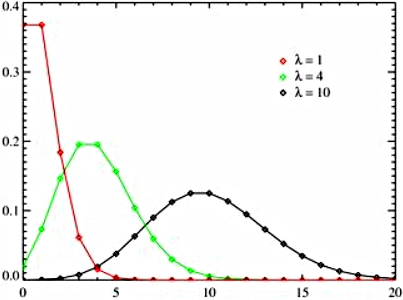
\includegraphics[width=8cm]{puasson.png}\par}

    Распределение Пуассона моделирует случайную величину $X$~--- ,,число событий, произошедших за заданное время``, при условии, что события происходят с заданной интенсивностью независимо друг от друга.
    
\end{frame}

\begin{frame}{Пример}{}

\end{frame}



\end{document}
